\chapter{Requirements specification}

\label{ch:requirements}
\lhead{Chapter 4. \emph{Requirements specification}}

This chapter describes the requirements for the product. These include both functional and non-functional requirements.
Functional requirements can be found in section \ref{section:functionalreq},
non-functional requirements in section \ref{section:nonfunctionalreq}.

Throughout this chapter both requirement's priority and complexity have a textual description which can be
\begin{itemize}
\item High
\item Medium (abbrev. Med)
\item Low
\end{itemize}

The use of such terms is described in table \ref{table:priorities} (priorities) and table \ref{table:complexity} (complexity).

\begin{table}[H]
\begin{center}
\begin{tabular}{ | c | p{12.5cm} | }
  \hline
  Priority & Description \\
  \hline\noalign{\smallskip}\noalign{\smallskip}\hline
  High & An essential requirement. The product \textbf{must fulfill} the requirement in order to be satisfactory. \\
  Medium & A useful requirement. The product \textbf{should fulfill} the requirement to maximise effectiveness. \\
  Low & A desiderabe requirement. The product \textbf{could fulfill} the requirement to be more interesting for certain stakeholders. \\
  \hline
\end{tabular}
\end{center}
\caption{Priority descriptions}
\label{table:priorities}
\end{table}

\begin{table}[H]
\begin{center}
\begin{tabular}{ | c | p{12.5cm} | }
  \hline
  Complexity & Description \\
  \hline\noalign{\smallskip}\noalign{\smallskip}\hline
  High & The requirement is difficult to implement. It will take a considerable amount of time. (more than 30 hours?) \\
  Medium & The requirement is moderately difficult. It will take some time. (from 10 to 30 hours?) \\
  Low & The requirement is easy and can be achieved in a short amount of time. (10h or less?) \\
  \hline
\end{tabular}
\end{center}
\caption{Complexity descriptions}
\label{table:complexity}
\end{table}

%-----

\section{Stakeholders}
\label{section:stakeholders}

This section contains the stakeholders of our system.
A short description of the role of each stakeholder is given, and what concerns they might have.

\subsection{Customer}
The customer is the one that is going to guide us to the solution he wants.
His concern is that we should maintain an effective and good communication with him, so he understands our progress.
We should also document the advancement we are making and have a clear system architecture for him.
His main concern is to get a working prototype of our system according to his requirements.

\subsection{Course evaluators}
The course evaluators are the one that are going to evaluate our project. 
Their concern is that the project should be well documented and understandable, and that all the deliveries should be on schedule.
Good communication is also of importance, and of course that we will learn something from the course.

\subsection{Our group}
We are going to write the report and implement our applications.
Our concern is to fulfil the requirements of our customer, finish the report and have a good presentation that reflects our work.

\subsection{Third party developers}
The third party developers are going to integrate our application to their system.
Their concern is that our integration platform should easily be connected with their applications.

\subsection{Users}
The users are the one that are going to use our Applications.
They are the users of our front-end, heart rate application and our weight application.
Their concern is that their data should be available for them, and visualized in an intuitive and comprehensible way.
They should be able to push heart rate data and weight data to our integration platform, without any difficulties.

%-----

\section{Funcional requirements}
\label{section:functionalreq}

This section describes the functional requirements for the product.
Each requirements has a priority which helps us identify the focus of our work.
Priorities can be reviewed based on customer's feedback. We tried to prioritize those requirements corresponding to the functionality of the system that the customer expressed most interest about. In order to better organize our workload we also assigned a \'difficulty\' to each requirement.

\textbf{Functional requirements for Integration platform}

\begin{table}[H]
\begin{center}
\begin{tabular}{ | c | p{9cm} | c | c | }
  \hline
  ID & Description & Difficulty & Priority\\
  \hline\noalign{\smallskip}\noalign{\smallskip}\hline
  FIP1	& The IP shall support REST endpoints for receiving heart rate data models expressed as JSON strings   & Med	& High \\
  FIP2	& The IP shall support REST endpoints for receiving weight data models expressed as JSON strings       & Med	& High \\
  FIP3	& The IP shall support REST endpoints for forwarding heart rate models (using JSON) to other systems.  & Med	& High \\
  FPI4	& The IP shall support REST endpoints for forwarding weight models (using JSON).                       & Med	& High \\
  \hline
\end{tabular}
\end{center}
\caption{Functional requirements for Integration platform}
\label{table:reqip}
\end{table}

\textbf{Functional requirements for the web frontend}

\begin{table}[H]
\begin{center}
\begin{tabular}{ | c | p{9cm} | c | c |}
  \hline
  ID & Description & Difficulty & Priority\\
  \hline\noalign{\smallskip}\noalign{\smallskip}\hline
  FW1	& The web frontend shall display the data stored by the Integration Platform using charts.	& Med	& High \\
  FW2	& The web frontend shall use Helsenorge color palette                                       & Low	& Low \\
  \hline
\end{tabular}
\end{center}
\caption{Functional requirements for the web frontend}
\label{table:reqfrontend}
\end{table}

\textbf{Functional requirements for Heart rate application}

\begin{table}[H]
\begin{center}
\begin{tabular}{ | c | p{9cm} | c | c |}
  \hline
  ID & Description & Difficulty & Priority\\
  \hline\noalign{\smallskip}\noalign{\smallskip}\hline
  FHR1	& The application shall measure user’s heart rate using the device camera    & Med	& High \\
  FHR2	& The application shall display the last measurement on the screen.          & Low	& Med \\
  FHR3	& The application shall forward the data to the IP using its REST endpoint.  & Med	& High \\
  \hline
\end{tabular}
\end{center}
\caption{Functional requirements for Heart rate application}
\label{table:reqheartrate}
\end{table}

\textbf{Functional requirements for Weight application}

\begin{table}[H]
\begin{center}
\begin{tabular}{ | c | p{9cm} | c | c |}
  \hline
  ID & Description & Difficulty & Priority\\
  \hline\noalign{\smallskip}\noalign{\smallskip}\hline
  FHV1	& The application shall fetch weight data from HealthVault.						      & Med	& High \\
  FHV2	& The application shall show the user the data it has fetched.              & Low	& Med \\
  FHV3	& The application shall forward the data to the IP using its REST endpoint. & Med	& High \\
  \hline
\end{tabular}
\end{center}
\caption{Functional requirements for Weight application}
\label{table:reqweight}
\end{table}

%-----

\section{Non-funcional requirements}
\label{section:nonfunctionalreq}

This section outlines non-functional requirements (quality attributes) for the product.
In order to provide a better overview, we have organized them in categories.

\begin{table}[H]
\begin{center}
\begin{tabular}{ | c | c |p{6.5cm} | c | c |}
  \hline
  ID & Category & Description & Difficulty & Priority\\
  \hline\noalign{\smallskip}\noalign{\smallskip}\hline
  NF1 & Documentation & The system shall be thoroughly documented, both at the code level and by the document ‘project report’.
  & High & High \\
  NF2 & Documentation & Although security and privacy are not requirements for the product they are important topics to be discussed in the documentation.
  & Med & High \\
  NF3 & Open-source	& The product shall be released under a permissive license approved by the product owner.
  & Low & High \\
  NF4 & Interoperability & The system shall provide a good degree of interoperability. Third party application developers should be put in the condition to develop third party (interoperable) solutions rapidly.
  & Med & High \\
  NF5 & Interoperability & A number of two-three prototype applications shall be developed in order to showcase the functionality of the system.
  & Med & High \\
  NF6 & Accessibility & The web-frontend should have a good degree of accessibility. It should have a rather simple design and use a user-provided palette.
  & Low & Low \\
  \hline
\end{tabular}
\end{center}
\caption{Non-functional requirements}
\label{table:reqnonfunc}
\end{table}

% -----

\section{Requirements Validation}
This section outlines the practices used to ensure requirements validity.

\textbf{Comprehensibility}\newline
It is important that requirements are expressed in a way that is understandable by the customer.
We have thus submitted a list of both functional and non-functional requirements of the system
to the customer for approval. Because requirements were subject to change due to the nature of the project
itself, the customer has reviewed them multiple times.

\textbf{Verifiability}\newline
It is crucial that a requirement can be tested. If a requirement can't be tested, it is not a valid requirement.
We have kept this in mind while formalising requirements.

%(Sommerville 7.3)
%How to ensure that a Requirements Document does define 
%the customers’ requirements (check against desirable 
%features)
%• Comprehensibility - do customers understand the 
%requirements?

%• Verifiability (testability) - can requirements be 
%realistically tested? If you cannot test it, it is not a 
%requirement!

%\textbf{Traceability}
%Requirements


%• Adaptability (changeability) - what is the impact of 
%changing a particular requirement?

%-----

\section{Use cases}

In this section we are going through the different use cases of our applications.
The section consists of use cases for the front-end, heart rate application and the weight application.

\subsection{Front-end}

The use case diagram for the front-end is shown in figure \ref{figure:use-case-diagram-front-end}.
From the use case diagram we see that the front-end has two main objectives.
The first one is to fetch data from our integration platform, and the second one is to visualize this data for the user.
In table \ref{table:use-case-view-data} a textual use case is given for the front-end.

\begin{figure}[H]
\centering
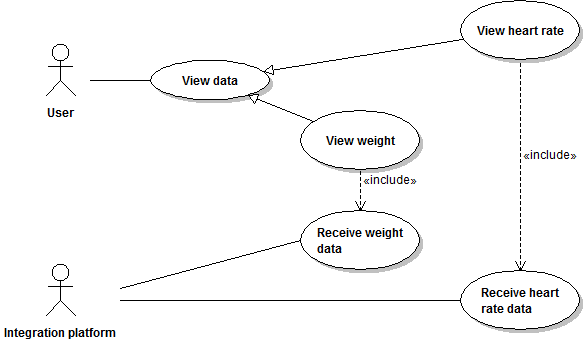
\includegraphics[scale=0.6]{../Figures/use-case-diagram-front-end.png}
\caption{Use case diagram - Front-end}
\label{figure:use-case-diagram-front-end}
\end{figure}

\begin{table}[H]
\begin{center}
\begin{tabular}{ l | p{10cm} }
  \hline
  \textbf{Use Case Element} & \textbf{Description} \\ \hline\hline
  Requirements & \hyperref[table:reqfrontend]{FW1}, \hyperref[table:reqip]{FIP3} and \hyperref[table:reqip]{FIP4}\\ \hline
  Application & Front-end \\ \hline
  Name & View data \\ \hline
  Description & Display all the data from the integration platform for the user. \\ \hline
  Actor & User and Integration Platform \\ \hline
  Precondition &
	\par 1. The integration platform has data about the current user.
	\par 2. The integration platform is online.
	\par 3. The user is using a computer with a web browser, that is connected to the internet.
	\\ \hline
  Basic Flow & 
  	\par 1. The user accesses the web page.
  	\par 2. Front-end requests data from the integration platform.
  	\par 3. Integration platform sends data to front-end.
  	\par 4. Front-end displays data to user.
  	\\ \hline
  Alternate Flows & 
  	\par 1A: The user wants to only view heart rate data.
  	\par\hspace{15pt} 1. The user clicks on \textit{Heart Rate} in the navigation bar.
  	\par 1B: The user wants to only view weight data.
  	\par\hspace{15pt} 1. The user clicks on \textit{Weight} in the navigation bar.
  \\ \hline
\end{tabular}
\end{center}
\caption{Textual use case - View data}
\label{table:use-case-view-data}
\end{table}

\subsection{Heart Rate Application}

A use case diagram for the heart rate application is given in figure \ref{figure:use-case-diagram-heart-rate}.
The main objectives of this application is to measure and send the data to the integration platform.

\begin{figure}[H]
\centering
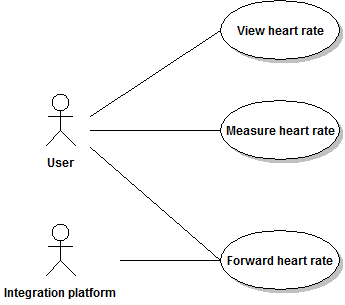
\includegraphics[scale=0.6]{../Figures/use-case-diagram-heart-rate.png}
\caption{Use case diagram - Heart rate application}
\label{figure:use-case-diagram-heart-rate}
\end{figure}

A textual use case for measuring and viewing the heart rate is given in table \ref{table:use-case-measure-heart-rate}.
Figure \ref{figure:use-case-diagram-measure-heart-rate} shows a use case diagram for the textual use case.

\begin{figure}[H]
\centering
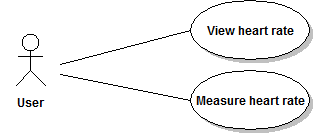
\includegraphics[scale=0.75]{../Figures/use-case-diagram-measure-and-view-heart-rate.png}
\caption{Use case diagram - Measure and view heart rate}
\label{figure:use-case-diagram-measure-heart-rate}
\end{figure}

\begin{table}[H]
\begin{center}
\begin{tabular}{ l | p{10cm} }
  \hline
  \textbf{Use Case Element} & \textbf{Description} \\ \hline\hline
  Requirements & \hyperref[table:reqheartrate]{FHR1} and \hyperref[table:reqheartrate]{FHR2} \\ \hline
  Application & Heart Rate Application \\ \hline
  Name & Measure and view heart rate \\ \hline
  Description & Measure the heart rate of the user and then view the measured data. \\ \hline
  Actor & User \\ \hline
  Precondition &
    \par 1. The users phone meets the requirements of the heart rate application.
  	\par 2. The application is installed on the users phone.
  	\par 3. The application is running on the users phone.
  \\ \hline
  Basic Flow & 
  	\par 1. The user places his finger on the camera of the phone.
  	\par 2. The user waits until the heart rate is shown on the display.
  	\par 3. The user views the heart rate.
  \\ \hline
  Alternate Flows & 
  	\par 1A: The user places his finger wrongly, which makes the measured data incorrect.
  	\par\hspace{15pt} 1. The user adjusts his finger.
  \\ \hline
\end{tabular}
\end{center}
\caption{Textual use case - Measure and view heart rate}
\label{table:use-case-measure-heart-rate}
\end{table}

Table \ref{table:use-case-send-heart-rate} gives a textual use case for sending the heart rate to the integration platform.
Figure \ref{figure:use-case-diagram-send-heart-rate} shows a use case diagram for the textual use case.

\begin{figure}[H]
\centering
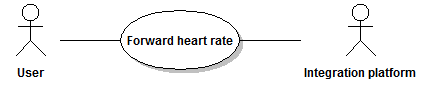
\includegraphics[scale=0.75]{../Figures/use-case-diagram-send-heart-rate.png}
\caption{Use case diagram - Send heart rate}
\label{figure:use-case-diagram-send-heart-rate}
\end{figure}

\begin{table}[H]
\begin{center}
\begin{tabular}{ l | p{10cm} }
  \hline
  \textbf{Use Case Element} & \textbf{Description} \\ \hline\hline
  Requirements & \hyperref[table:reqheartrate]{FHR3} and \hyperref[table:reqip]{FIP1} \\ \hline
  Application & Heart Rate Application \\ \hline
  Name & Send heart rate \\ \hline
  Description & Send the measured heart rate to the integration platform. \\ \hline
  Actor & User and Integration Platform \\ \hline
  Precondition &
    \par 1. The user has measured his/hers heart rate through the application.
    \par 2. The phone is connected to the internet.
    \par 3. The integration platform is online.
  \\ \hline
  Basic Flow & 
  	\par 1. The user clicks on \textit{Send}.
  	\par 2. The application sends the data to the integration platform.
  	\par 3. The integration platform receives the data.
  \\ \hline
\end{tabular}
\end{center}
\caption{Textual use case - Send heart rate}
\label{table:use-case-send-heart-rate}
\end{table}

\subsection{Weight Application}

The goal of the weight application is to retrieve weight data from HaulthVault and forward it to our integration platform.
Figure \ref{figure:use-case-diagram-weight} shows the main use case diagram for the application.

\begin{figure}[H]
\centering
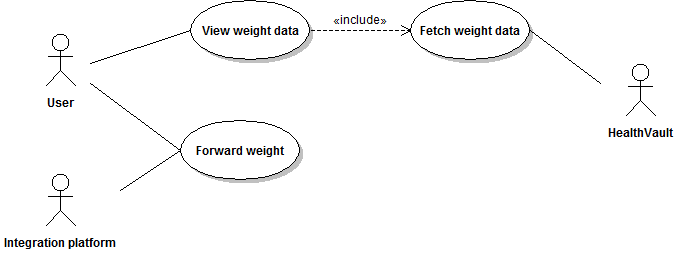
\includegraphics[scale=0.6]{../Figures/use-case-diagram-weight.png}
\caption{Use case diagram - Weight application}
\label{figure:use-case-diagram-weight}
\end{figure}

In figure \ref{figure:use-case-diagram-view-weight} a use case diagram is given for fetching and viewing the weight data.
Table \ref{table:use-case-view-weight-data} gives a textual use case for the use case diagram.

\begin{figure}[H]
\centering
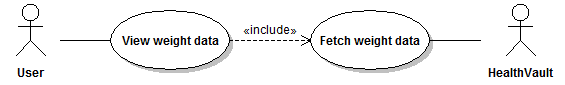
\includegraphics[scale=0.75]{../Figures/use-case-diagram-view-weight.png}
\caption{Use case diagram - View weight data}
\label{figure:use-case-diagram-view-weight}
\end{figure}

\begin{table}[H]
\begin{center}
\begin{tabular}{ l | p{10cm} }
  \hline
  \textbf{Use Case Element} & \textbf{Description} \\ \hline\hline
  Requirements & \hyperref[table:reqweight]{FHV1} and \hyperref[table:reqweight]{FHV2}\\ \hline
  Application & Weight Application \\ \hline
  Name & View weight data \\ \hline
  Description & Fetch the weight data from HealthVault and display it for the user. \\ \hline
  Actor & User and HealthVault \\ \hline
  Precondition &
    \par 1. The users phone meets the requirements of the weight application.
  	\par 2. The application is installed on the users phone.
  	\par 3. The application is running on the users phone.
  	\par 4. The application is connected to the internet.
  \\ \hline
  Basic Flow & 
  	\par 1. The user writes his email to HealthVault into the email field.
  	\par 2. The user writes his password to HealthVault into the password field.
  	\par 3. The user clicks on a button to login.
  	\par 4. The application shows the data for the user.
  	\par 5. The user views the data.
  \\ \hline
  Alternate Flows & 
  	\par 3A: The user inputs an invalid password or email.
  	\par\hspace{15pt} 1. The user has to go back to step 1 and start over again.
  \\ \hline
\end{tabular}
\end{center}
\caption{Textual use case - View weight data}
\label{table:use-case-view-weight-data}
\end{table}

Table \ref{table:use-case-send-weight-data} gives a textual use case for sending the weight data to our integration platform.
Figure \ref{figure:use-case-diagram-send-weight} displays a use case diagram for the textual use case.

\begin{figure}[H]
\centering
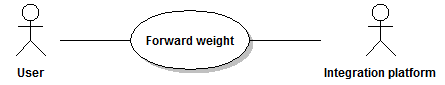
\includegraphics[scale=0.75]{../Figures/use-case-diagram-send-weight.png}
\caption{Use case diagram - Send weight data}
\label{figure:use-case-diagram-send-weight}
\end{figure}

\begin{table}[H]
\begin{center}
\begin{tabular}{ l | p{10cm} }
  \hline
  \textbf{Use Case Element} & \textbf{Description} \\ \hline\hline
  Requirements & \hyperref[table:reqweight]{FHV3} and \hyperref[table:reqip]{FIP2}\\ \hline
  Application & Weight Application \\ \hline
  Name & Send weight data \\ \hline
  Description & Send the weight data from the phone application into the integration platform. \\ \hline
  Actor & User and Integration Platform \\ \hline
  Precondition &
    \par 1. The user has acquired the weight data through the weight application.
    \par 2. The integration platform is online.
  \\ \hline
  Basic Flow & 
  	\par 1. The user presses the \textit{Send} button.
  	\par 2. The Integration platform receives the data.
  \\ \hline
\end{tabular}
\end{center}
\caption{Textual use case - Send weight data}
\label{table:use-case-send-weight-data}
\end{table}



\section{Test plan}

Most of the testing was performed manually.
Since the product consisted of two Android applications and a Spring
